\documentclass[preprint,12pt,authoryear=false]{elsarticle}

\usepackage[utf8]{inputenc}
\usepackage[T1]{fontenc}
\usepackage{lmodern}
\usepackage[a4paper,top=22mm,bottom=24mm,left=28mm,right=28mm]{geometry}
\usepackage{amsmath,amssymb}
\usepackage{graphicx}
\usepackage{booktabs}
\usepackage{longtable}
\usepackage{tabularx}
\usepackage{multirow}
\usepackage{xcolor}
\usepackage{tikz}
\usetikzlibrary{positioning,arrows.meta,calc}
\usepackage[hidelinks]{hyperref}
\usepackage{lineno}
\linenumbers

% ---------------------------------------------------------------
% Author notes. Every \pendente{} marks work that still needs new
% data or a decision by the authors. Remove all of them before
% submission (search for "PENDENTE").
% ---------------------------------------------------------------
\newcommand{\pendente}[1]{\textcolor{red}{\textbf{[PENDENTE:} #1\textbf{]}}}

\newcommand{\PM}{TF-PM}
\newcommand{\ST}{TF-ST}
\newcommand{\FC}{TF-FC}
\newcommand{\MSR}{TF-MSR}

\journal{Information and Software Technology}
\makeatletter\def\ps@pprintTitle{\let\@oddhead\@empty\let\@evenhead\@empty\def\@oddfoot{\hfill\thepage\hfill}\let\@evenfoot\@oddfoot}\makeatother

\begin{document}

\begin{frontmatter}

\title{Process Mining, Stochastic Modelling, and Forecasting of Software Development Processes: A Systematic Mapping Study}

\author[pucpr]{Rodrigo Almeida de Oliveira\corref{cor1}}
\ead{rodrigo.almeida1@pucpr.edu.br}
\author[pucpr]{Juliano de Paulo Ribeiro}
\ead{juliano.ribeiro@pucpr.edu.br}
\author[pucpr]{Edson Emilio Scalabrin}
\ead{scalabrin@ppgia.pucpr.br}
\cortext[cor1]{Corresponding author.}
\affiliation[pucpr]{organization={Pontifícia Universidade Católica do Paraná (PUCPR), Graduate Program in Informatics (PPGIa)},
  city={Curitiba}, state={PR}, country={Brazil}}

\begin{abstract}\small
\textbf{Context.} Software repositories record development as time-stamped events. Process mining (PM), stochastic modelling, and forecasting of process metrics exploit such traces, largely independently.
\textbf{Objective.} To map the primary studies that apply these techniques to software development data, to characterise how the three lines have evolved, and to measure how far they have been integrated.
\textbf{Method.} A systematic mapping study reported against SEGRESS. Five libraries and one citation-search iteration gave 5,783 unique records (12 April 2026). A language model served as a first-pass screening aid; every record it excluded or left undecided was re-screened by two human reviewers. Studies were classified into four technique and data families and into four integration levels (L0--L3).
\textbf{Results.} The corpus contains 435 studies published between 1994 and 2026, all classified. Stochastic modelling (55.4\%) dominated until 2013; process mining (39.8\%) has dominated since 2014. The two lines meet in 10 studies. Forecasting appears in 28.0\% of the studies, mostly paired with stochastic models (95 studies) and rarely with process mining (9). One study combines all three families (L2), and none couples them through specified interfaces evaluated end-to-end (L3).
\textbf{Conclusion.} The field is fragmented along community lines rather than short of techniques. Process-aware stochastic forecasting, in which mined process structure parameterises a stochastic forecast, is the least explored combination. A four-direction agenda is proposed.
\end{abstract}

\begin{highlights}
\item 435 studies apply process mining, stochastic models or forecasting to SDLC data.
\item Stochastic modelling dominated until 2013; process mining has dominated since.
\item Process mining and stochastic modelling meet in 10 of 435 studies.
\item One study combines all three; none couples them with end-to-end evaluation.
\item Corpus, classification, and screening records are openly available.
\end{highlights}

\begin{keyword}
Systematic mapping study \sep Process mining \sep Stochastic modelling \sep Software process forecasting \sep Mining software repositories
\end{keyword}

\end{frontmatter}

% =================================================================
\section{Introduction}\label{sec:intro}

Software organisations routinely need to answer forecasting questions about their own development process: when a feature will be delivered, how long an issue will remain open, or whether a release will slip. The data needed to answer them already exists as a by-product of everyday work. Commits, issue transitions, pull requests, code reviews, and CI/CD executions are all time-stamped events.

Three research communities have developed techniques that can exploit these traces, largely independently of one another. Process mining (PM) discovers, checks, and enhances process models from event logs, and has been applied to software repositories since the work of Cook and Wolf~\cite{cook1995,cook1998} and Rubin et al.~\cite{rubin2007}. Stochastic modelling, including Markov chains, stochastic Petri nets, and Monte Carlo simulation, has a long tradition in software reliability and process simulation~\cite{whittaker1994,ali2014}. Machine-learning-based prediction dominates mining-software-repositories research on defects, effort, and outcomes~\cite{kagdi2007,hall2012} and, in business process management, predictive process monitoring~\cite{marquez2018}.

Combining the three is attractive because each covers a weakness of the others. PM provides an empirically grounded process structure. Stochastic models turn that structure into probability distributions over future paths and durations. Learned models can correct systematic errors using context features. Whether such combinations have been built, and on which data, is not known.

\paragraph{Related secondary studies}
Existing secondary studies each cover one side of this space. Predictive process monitoring has been surveyed and benchmarked for outcome prediction~\cite{teinemaa2019}, remaining-time prediction~\cite{verenich2019}, deep-learning methods~\cite{ramamaneiro2023}, and in general~\cite{marquez2018}, but on business event logs rather than software development processes. General mappings of process mining applications~\cite{garcia2019,thiede2018} treat software engineering as one domain among many and do not address forecasting. Within software engineering, secondary studies have covered process simulation modelling~\cite{zhang2010,ali2014}, process mining of FLOSS event logs~\cite{mukala2015}, software process mining with Petri nets~\cite{thamizharasan2016}, continuous software monitoring backed by process mining~\cite{stepanov2026}, repository mining~\cite{kagdi2007}, and defect prediction~\cite{hall2012}. None maps the joint use of process mining, stochastic modelling, and forecasting on software development data.

\paragraph{Contributions}
This article reports a systematic mapping study of that intersection. Its contributions are:
\begin{enumerate}
\item a corpus of 435 primary studies, openly available with the screening and classification records;
\item a classification of the studies into four technique and data families and into four integration levels, with the evolution of each family over three decades; and
\item an analysis of the gaps between the three research lines, from which we derive a four-direction research agenda.
\end{enumerate}

The review was motivated by the authors' own work on an integrated forecasting pipeline. We report this because it is a potential source of bias in how the integration levels were defined and read; the definitions in Section~\ref{sec:classification} are therefore stated without reference to any particular architecture, and the threat is discussed in Section~\ref{sec:threats}.

Section~\ref{sec:method} describes the review protocol, Section~\ref{sec:selection} the search and selection results, Section~\ref{sec:results} the answers to the research questions, Section~\ref{sec:discussion} the discussion and research agenda, Section~\ref{sec:threats} the threats to validity, and Section~\ref{sec:conclusion} concludes.

% =================================================================
\section{Review Protocol}\label{sec:method}

We follow the mapping guidelines of Petersen et al.~\cite{petersen2015}, the guidelines of Kitchenham and Charters~\cite{kitchenham2007}, and the snowballing procedure of Wohlin~\cite{wohlin2014}, and report against SEGRESS~\cite{segress}. The mapping protocol was not registered in advance. The completed SEGRESS checklist is in the supplementary material.

\subsection{Research questions}\label{sec:rqs}

\begin{description}
\item[RQ1] How has research applying process mining, stochastic modelling, or forecasting to software development data evolved over time?
\item[RQ2] Which technique families, and which combinations of them, do the studies use?
\item[RQ3] Which SDLC phases, event-log sources, and specific techniques do the studies address?
\item[RQ4] To what extent are process mining, stochastic modelling, and forecasting integrated, and which gaps remain?
\end{description}

RQ1 and RQ2 characterise the corpus. RQ3 describes what the studies analyse and with which algorithms. RQ4 addresses the motivating question of this review.

\pendente{RQ3 só pode ser respondida após a extração humana dos campos fase do SDLC, fonte e construção do event log, algoritmo de PM, método estocástico e alvo da previsão (ver Seção~\ref{sec:rq3}). A extração anterior, feita pelo LLM, teve 0\% de concordância exata com o avaliador humano e não pode ser usada. Se a extração não for feita, retirar RQ3 do artigo.}

\subsection{Search strategy}\label{sec:search}

The automated search covered five digital libraries: IEEE Xplore, ACM Digital Library, Scopus, Web of Science, and SpringerLink. The strings were built from a PICO decomposition adapted to software engineering. The population is the software engineering context (software development, SDLC, DevOps, CI/CD, issue tracking, version control, code review). The intervention is the analytical technique (process mining, process discovery, conformance checking, predictive process monitoring, Markov chain, Monte Carlo, stochastic Petri net). The outcome is a forecast or a process model (lead time, cycle time, remaining time, throughput). There is no comparison facet.

Three complementary term lists were derived: a principal string joining population and intervention; a complementary string for studies that use MSR terminology without canonical PM terms; and a frontier string for the intersection of stochastic methods and PM in software contexts. They were adapted to each library, giving 25 exports (Table~\ref{tab:search}). All searches were run on 12 April 2026, with a publication window from 1 January 1994 (Whittaker and Thomason~\cite{whittaker1994}) to that date. Publications dated 2026 are therefore partial-year coverage. The shared term lists are given in \ref{app:strings}; every database-specific string is in the replication package.

\pendente{Três strings do Scopus contêm os títulos literais de artigos do conjunto de controle (V6, V8, V9). Opção A: retirar os títulos, rodar as strings de novo e atualizar as Tabelas~\ref{tab:search} e~\ref{tab:selection}. Opção B: manter, deixando a declaração da Seção~\ref{sec:threats-search}, e validar a busca com um conjunto de teste independente.}

\pendente{Nenhuma string principal tem bloco de forecasting/ML em repositórios (por exemplo ``bug fix time'', ``issue resolution time'', ``effort estimation'', ``machine learning'')~\cite{panjer2007,giger2010}. Rodar esse bloco nas cinco bases e incorporar os resultados ao corpus. A busca suplementar no Scopus de 31/10/2026 (165 registros, 19 includes por título) deve ser incorporada ou descartada de vez.}

\begin{table}[t]
\centering\small
\caption{Search ledger by source. All exports were retrieved on 12 April 2026. Unique records are counted once, under the source that supplied the retained copy.}\label{tab:search}
\begin{tabular}{lllrr}
\toprule
Source & Field searched & Exports & Raw records & Unique \\
\midrule
Scopus & TITLE-ABS-KEY & 6 & 2,377 & 1,852 \\
SpringerLink & Simplified search & 10 & 2,884 & 1,543 \\
IEEE Xplore & All metadata & 17 batches & 1,386 & 1,263 \\
Web of Science & Topic (TS) & 4 & 997 & 514 \\
ACM DL & Abstract & 2 + 1 export & 96 & 34 \\
Snowballing & -- & 1 iteration & 595 & 575 \\
Control set & -- & -- & 12 & 2 \\
\midrule
Total & & & 8,347 & 5,783 \\
\bottomrule
\end{tabular}
\end{table}

\paragraph{Snowballing}
One iteration of backward and forward snowballing was run over 400 source DOIs and retrieved 595 records. A candidate was kept when its title or abstract contained one PM or stochastic term and one software-engineering term.

\pendente{O procedimento acima não segue Wohlin~\cite{wohlin2014}: os 400 DOIs-fonte não são os estudos incluídos, backward e forward não estão separados e não houve critério de saturação. Refazer o snowballing a partir dos 435 estudos, separando backward e forward e iterando até nenhum estudo novo aparecer, e informar as contagens por iteração. Sem isso, descrever o procedimento como ``one iteration of citation search'' e não como snowballing de Wohlin.}

\paragraph{Control set}
Ten known studies (Table~\ref{tab:control}) were used to check that the strings retrieve relevant work. All ten were retrieved. Because the ten were known when the strings were written, this check does not estimate the sensitivity of the search.

\begin{table}[t]
\centering\small
\caption{Control studies for the search-string check.}\label{tab:control}
\footnotesize
\begin{tabularx}{\textwidth}{llXl}
\toprule
\# & Study & Rationale & Retrieved via \\
\midrule
V1 & Cook \& Wolf (1998) & Seminal PM in SE & ACM \\
V2 & Rubin et al. (2007) & PM framework for software processes & Scopus \\
V3 & Poncin et al. (2011) & PM and MSR & IEEE \\
V4 & Caldeira \& Cardoso (2019) & PM for software process assessment & IEEE \\
V5 & Lemos et al. (2011) & PM for software process management & IEEE \\
V6 & Whittaker \& Thomason (1994) & Markov models in software testing & Scopus \\
V7 & Tax et al. (2017) & Predictive process monitoring (BPM) & Control set \\
V8 & Rogge-Solti \& Weske (2015) & Stochastic PM forecasting & Scopus \\
V9 & Rozinat et al. (2009) & From PM to simulation & Control set \\
V10 & Gupta \& Sureka (2017) & Multi-repository PM in SE & ACM \\
\bottomrule
\end{tabularx}
\end{table}

\subsection{Eligibility criteria}\label{sec:criteria}

Table~\ref{tab:criteria} lists the criteria. The unit of counting is the publication~\cite{petersen2015}. Duplicate records of the same publication are merged. A conference paper and its later extension are both retained when each satisfies the criteria independently; there are two such pairs in the corpus, and counting them once would change no reported percentage by more than one point.

A study is included when it satisfies IC1--IC3 and at least one of the content criteria IC4a--IC4d, and none of EC1--EC5. The four content criteria define the four families used throughout the article: \PM{} (IC4a), \ST{} (IC4b), \FC{} (IC4c), and \MSR{} (IC4d). \PM{}, \ST{}, and \FC{} are technique families; \MSR{} describes the data source.

\pendente{IC4b e IC4c, como estão, aceitam modelos Markovianos de teste estatístico e modelos de crescimento de confiabilidade (``defect rates''). Esses modelos descrevem o produto, não o processo de desenvolvimento, e provavelmente formam boa parte dos 94 estudos ST+FC de 1997--2013. Decidir: (a) mantê-los, declarando o escopo amplo; ou (b) acrescentar um EC (``model of product reliability, not of the development process'') e reclassificar.}

\begin{table}[t]
\centering\small
\caption{Inclusion and exclusion criteria.}\label{tab:criteria}
\begin{tabularx}{\textwidth}{llX}
\toprule
Type & ID & Criterion \\
\midrule
\multirow{7}{*}{Inclusion}
 & IC1 & Published between 1 January 1994 and 12 April 2026. \\
 & IC2 & Written in English. \\
 & IC3 & Peer-reviewed journal article, conference paper, or workshop paper of at least four pages. \\
 & IC4a & Applies process mining (discovery, conformance checking, predictive process monitoring) to software development artefacts (commits, issues, pull requests, CI/CD logs, bug trackers, version control). \\
 & IC4b & Uses stochastic models (Markov chains, Monte Carlo, stochastic Petri nets, absorbing chains) to analyse software development processes or workflows. \\
 & IC4c & Proposes or evaluates forecasting of software process metrics (lead time, cycle time, remaining time, throughput, defect rates) from event logs or repository data. \\
 & IC4d & Mines software repositories (GitHub, Jira, version control, CI/CD platforms) to discover, analyse, or improve software process models. \\
\midrule
\multirow{5}{*}{Exclusion}
 & EC1 & Application domain exclusively outside software development, without demonstrated relevance to SDLC processes. \\
 & EC2 & Software is only the implementation platform; the analysed process is not a software development process. \\
 & EC3 & Purely algorithmic or theoretical contribution without empirical evaluation in a software development context. \\
 & EC4 & Secondary study not specifically addressing PM or stochastic methods in software engineering. \\
 & EC5 & Record cannot be judged on the obtainable evidence: full text not retrievable (EC5a), no abstract and no full text (EC5b), or decision-critical information absent (EC5c). \\
\bottomrule
\end{tabularx}
\end{table}

\subsection{Selection process}\label{sec:selection-process}

Selection had three steps.

\paragraph{Step 1: language-model-assisted first pass}
A language model (claude-haiku-4-5-20251001, Anthropic Message Batches API) screened every unique record against IC4a--IC4d and EC1--EC4, returning \emph{include}, \emph{exclude}, or \emph{maybe} with a short rationale. Records marked include or maybe were forwarded to a second, stricter pass on the title and abstract (\emph{include}, \emph{exclude}, or \emph{pending}). Abstracts missing from the exports were recovered beforehand from Semantic Scholar, OpenAlex, CORE, and Crossref. The prompts, JSON schemas, and per-record decisions are in the replication package.

\paragraph{Step 2: human verification of the first pass}
Two raters, blind to the model's decisions and to each other, judged a stratified random sample of 177 second-pass decisions against Table~\ref{tab:criteria}. Inter-rater agreement before consensus was $\kappa = 0.654$. Against the consensus, the first pass retained 29 of 46 eligible sampled studies (Recall 0.630; Wilson 95\% CI 0.486--0.755). For the records of the second screening batch, stratified samples of the model's non-includes gave an estimated Recall of 0.563. The success criterion fixed before this check was a Recall of at least 0.90. Because it was not met, the first pass is used here only to prioritise records, and Step~3 re-screened every record it had not included.

The success criterion (Recall $\geq 0.90$), the sampling plan, and the escalation rules for this check were fixed in a written pre-registration dated 2026-10-06 (\texttt{PREREGISTRATION\_round2\_validation.md} in the project repository), before round-2 human judgements were collected. \pendente{Depositar esse pré-registro em OSF ou Zenodo e substituir esta frase pelo DOI/URL público.}

\paragraph{Step 3: human re-screen and check of the includes}
Two reviewers screened all 4,005 records the first pass had excluded or left undecided, including 611 records closed without a decision for lack of an abstract. They also checked every first-pass include against the criteria. The re-screen identified 188 eligible records, which after de-duplication and a final eligibility check added 150 studies. The check of the includes removed 32 studies whose title and abstract did not support inclusion.

For the large auxiliary strata S1 (title/abstract excludes; $n = 2383$ in the escalation sheet) and S3 (records previously closed without an abstract; $n = 551$), the working spreadsheets carried pre-filled suggestion columns (\texttt{sug\_*}). Suggestions came from two sources: (i)~a typed keyword heuristic aligned with Table~\ref{tab:criteria}, and (ii)~in part of S1 only, batch agent pre-classifications merged as \texttt{preclass\_source=agent\_batches\_*}. These suggestions are \emph{not} the Step~1 Haiku model. In the archived S1 and S3 sheets, however, the official \texttt{decision} column equals \texttt{sug\_decision} on every row (100\%), so rater judgements are not separable from the suggestion and no trustworthy Step~3 $\kappa$ can be computed from those files alone. A stratified blind re-screen without suggestions (all 47 S1/S3 includes plus 70 random excludes; seed 20261111) is under way to report agreement and $\kappa$; see the Phase~2 protocol in the replication materials.

\pendente{Após a re-triagem cega: informar $\kappa$ A vs B e a concordância com a decisão original; se houver flips de include, atualizar o corpus.}

\subsection{Data extraction and classification}\label{sec:classification}

For each included study we recorded the bibliographic data, the families it satisfies (\PM{}, \ST{}, \FC{}, \MSR{}), and its integration level. The integration level depends only on the three technique families:

\begin{description}
\item[L0] At most one technique family.
\item[L1] Exactly two technique families.
\item[L2] All three technique families in the same study, with stages evaluated separately or connected without specified interfaces.
\item[L3] All three technique families coupled through specified data interfaces, in which the output of each stage is the input of the next, and evaluated end-to-end on software development data.
\end{description}

L0 and L1 follow mechanically from the family codes. Telling L2 from L3 requires reading the study's evaluation; this was needed for one study only (Section~\ref{sec:rq4}).

Families were first proposed by the language model from the title, abstract, and, where available, the PDF. The authors then reviewed them as follows. Every study with two technique families ($n = 111$) was re-read for a missing third family; a subset was read by two authors with full agreement, and no study changed level. Studies added by the re-screen were classified by the authors. The 76 title-only records from the re-screen were resolved from abstract or PDF: 55 were classified into the corpus and 21 were excluded (out of scope or EC5b), leaving 435 included studies, all classified.

A stratified sample of 55 L0 studies (period $\times$ family) was re-coded by one author against title/abstract/PDF. Agreement with the LLM family codes was 55/55 (0\% error on this sample). A second coder for $\kappa$ was not run; that remains an optional strengthening of the audit.

\pendente{Extração para RQ3 e para o mapa de venues: fase do SDLC, fonte do event log, construção do log (manual, semi, automática), algoritmo de PM, método estocástico, técnica de ML, alvo da previsão, tipo de validação, research type (Wieringa et al.~\cite{wieringa2006}) e venue. Dois extratores humanos, ou um extrator e um verificador numa amostra com $\kappa$ reportado.}

% =================================================================
\section{Search and Selection Results}\label{sec:selection}

The search returned 8,347 records. Cross-source de-duplication by DOI, followed by fuzzy title matching (Levenshtein similarity $\geq 0.9$) for records without a DOI, removed 2,564 duplicates and left 5,783 unique records. For practical reasons the first pass ran in two batches. The primary batch contained the records from the principal Scopus, IEEE Xplore, and ACM queries; the second contained the remaining records (SpringerLink, Web of Science, snowballing, and the other IEEE and ACM exports). Table~\ref{tab:selection} gives the outcome of each step, and Figure~\ref{fig:prisma} the overall flow.

\begin{table}[t]
\centering\small
\caption{Outcome of the selection steps. Batch identifier lists overlap by 364 papers recorded under different identifiers; their union is the 5,783 unique records.}\label{tab:selection}
\footnotesize
\begin{tabular}{lrr}
\toprule
Step & Primary batch & Second batch \\
\midrule
Records screened (Step 1, title/abstract) & 2,340 & 3,807 \\
\quad include / maybe & 111 / 775 & 232 / 1,151 \\
Second pass (Step 1) & 886 & 1,383 \\
\quad include & 169 & 212 + 23 \\
\midrule
First-pass includes, distinct after de-duplication & \multicolumn{2}{c}{340} \\
\quad removed: published before 1994 (IC1) & \multicolumn{2}{c}{2} \\
\quad removed by the human check of includes (Step 3) & \multicolumn{2}{c}{32} \\
Records re-screened by humans (Step 3) & \multicolumn{2}{c}{4,005} \\
\quad eligible, new after de-duplication & \multicolumn{2}{c}{168} \\
\quad removed in the final eligibility check & \multicolumn{2}{c}{18} \\
\midrule
Screened includes before title-only resolution & \multicolumn{2}{c}{306 + 150 = 456} \\
\quad removed resolving title-only (out of scope / EC5b) & \multicolumn{2}{c}{21} \\
Included studies (all classified) & \multicolumn{2}{c}{435} \\
\bottomrule
\end{tabular}
\end{table}

\begin{figure}[t]
\centering
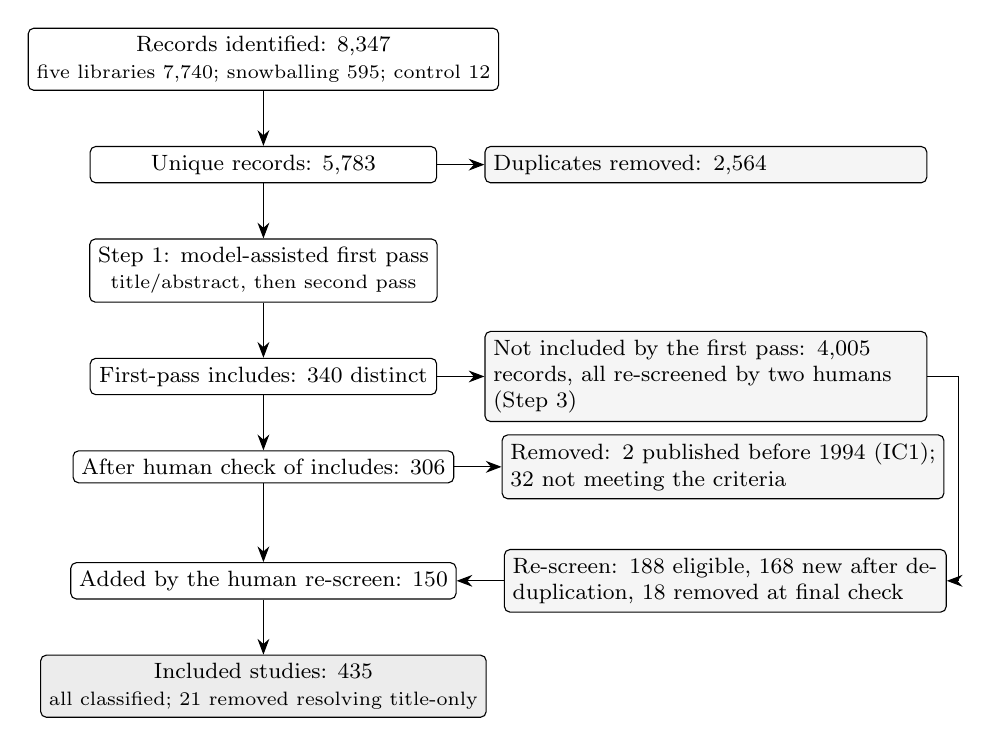
\begin{tikzpicture}[
  box/.style={draw, rounded corners=2pt, align=center, font=\footnotesize, minimum width=4.4cm, inner sep=3pt},
  side/.style={draw, rounded corners=2pt, align=left, font=\footnotesize, text width=5.4cm, inner sep=3pt, fill=gray!8},
  arr/.style={-{Stealth[length=2mm]}, thin}, node distance=7mm]
\node[box] (id) {Records identified: 8,347\\ \scriptsize five libraries 7,740; snowballing 595; control 12};
\node[box, below=of id] (dd) {Unique records: 5,783};
\node[box, below=of dd] (s1) {Step 1: model-assisted first pass\\ \scriptsize title/abstract, then second pass};
\node[box, below=of s1] (inc1) {First-pass includes: 340 distinct};
\node[box, below=of inc1] (chk) {After human check of includes: 306};
\node[box, below=10mm of chk] (add) {Added by the human re-screen: 150};
\node[box, below=of add, fill=gray!15] (fin) {Included studies: 435\\ \scriptsize all classified; 21 removed resolving title-only};
\node[side, right=6mm of dd] (dup) {Duplicates removed: 2,564};
\node[side, right=6mm of inc1] (ex1) {Not included by the first pass: 4,005 records, all re-screened by two humans (Step 3)};
\node[side, right=6mm of chk] (rm) {Removed: 2 published before 1994 (IC1); 32 not meeting the criteria};
\node[side, right=6mm of add] (rm2) {Re-screen: 188 eligible, 168 new after de-duplication, 18 removed at final check};
\draw[arr] (id) -- (dd); \draw[arr] (dd) -- (s1); \draw[arr] (s1) -- (inc1); \draw[arr] (inc1) -- (chk);
\draw[arr] (chk) -- (add); \draw[arr] (add) -- (fin);
\draw[arr] (dd) -- (dup); \draw[arr] (inc1) -- (ex1); \draw[arr] (chk) -- (rm);
\draw[arr] (ex1.east) -- ++(4mm,0) |- (rm2.east); \draw[arr] (rm2) -- (add);
\end{tikzpicture}
\caption{PRISMA 2020 flow~\cite{page2021} of the study selection.}\label{fig:prisma}
\end{figure}

The second-pass exclusions in the primary batch ($n = 717$) were driven by EC3 (232; algorithmic or theoretical contributions without software engineering evaluation), EC1 (205; mostly generic business process management), EC5 (145), EC2 (110), and EC4 (60). A study may trigger more than one criterion. The size of EC3 indicates a sizeable body of PM and stochastic research not yet evaluated on software development data.

% =================================================================
\section{Results}\label{sec:results}

The corpus contains 435 studies, all classified. All percentages below are computed on these 435 studies. The full list is in \ref{app:studies}.

\subsection{RQ1: Evolution over time}\label{sec:rq1}

The 435 studies span 1994--2026 (Figure~\ref{fig:years}). Since 2006 most years contribute 13 to 26 studies, with dips in 2013 (3), 2020 (10), and 2025 (6); 2026 is a partial year. In total, 213 studies (49.0\%) appeared in 2015--2026.

The 2013 dip (3 included studies) is not explained by a missing harvest year: the unique-record pool contains 263 records dated 2013, comparable to 227 (2012) and 249 (2014). The trough therefore arises downstream of search (screening/eligibility). A dedicated audit of 2013 excludes remains desirable but is not required to rule out an indexing gap.

\begin{figure}[t]
\centering
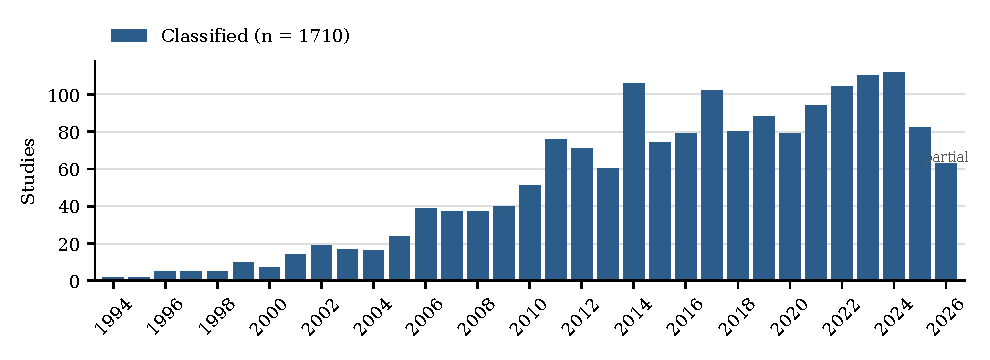
\includegraphics[width=\textwidth]{figs/years.pdf}
\caption{Included studies per publication year ($n = 435$).}\label{fig:years}
\end{figure}

The composition of the field changed sharply around 2014 (Figure~\ref{fig:bubble}). Until 2013 the corpus is dominated by stochastic models: 91\% of the studies of 1994--2005 and 74\% of 2006--2013 carry \ST{}. From 2014 process mining takes over, with \PM{} in 60\% of the studies of 2014--2019 and 59\% of 2020--2026, while \ST{} falls to about a third. Repository mining (\MSR{}) grows steadily, from 3\% to 39\% of the studies of each period. The share of forecasting (\FC{}) is roughly stable, between 22\% and 36\%.

\begin{figure}[t]
\centering
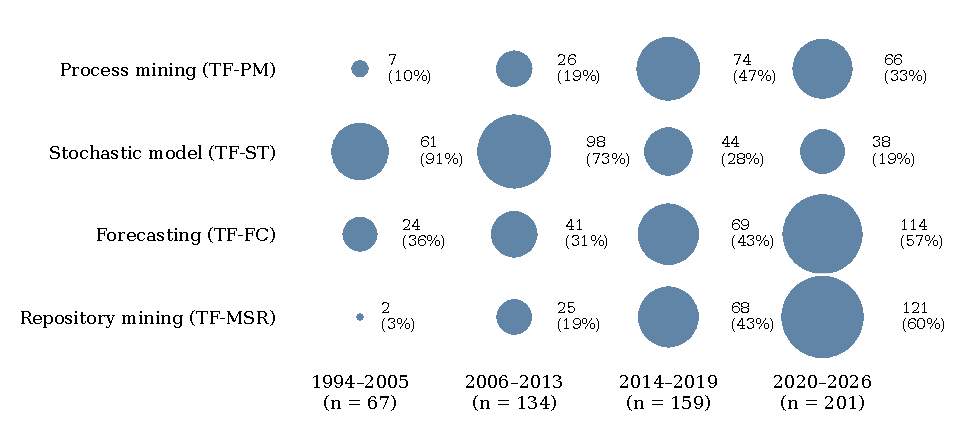
\includegraphics[width=0.92\textwidth]{figs/bubble.pdf}
\caption{Technique and data families by period ($n = 435$). Bubble area is proportional to the number of studies; the percentage is the share of the period's studies that carry the family. Families are not exclusive.}\label{fig:bubble}
\end{figure}

\pendente{Acrescentar a distribuição por tipo de publicação (periódico, conferência, workshop) e os venues mais frequentes, a partir da extração da Seção~\ref{sec:classification}.}

\subsection{RQ2: Technique families and their combinations}\label{sec:rq2}

Of the 435 studies, 241 (55.4\%) carry \ST{}, 173 (39.8\%) \PM{}, 122 (28.0\%) \FC{}, and 104 (23.9\%) \MSR{}. Table~\ref{tab:combos} shows how the three technique families combine.

\begin{table}[t]
\centering\small
\caption{Combinations of the three technique families in the 435 studies. Each study appears in exactly one row. The \MSR{} column counts studies of that row that also mine repositories.}\label{tab:combos}
\begin{tabular}{lrrrc}
\toprule
Combination & Studies & \% & with \MSR{} & Median year \\
\midrule
\PM{} only & 155 & 35.6 & 63 & 2018 \\
\ST{} only & 137 & 31.5 & 16 & 2009 \\
\ST{} + \FC{} & 94 & 21.6 & 2 & 2010 \\
\FC{} only & 19 & 4.4 & 6 & 2018 \\
\PM{} + \ST{} & 9 & 2.1 & 1 & 2016 \\
None (\MSR{} only) & 12 & 2.8 & 12 & 2017 \\
\PM{} + \FC{} & 8 & 1.8 & 4 & 2018 \\
\PM{} + \ST{} + \FC{} & 1 & 0.2 & 0 & 2025 \\
\midrule
Total & 435 & 100.0 & 104 & \\
\bottomrule
\end{tabular}
\end{table}

Two clusters account for 89\% of the corpus and barely overlap. The first is process mining, often on repository data: 155 studies use PM without stochastic modelling or forecasting, and 63 of them mine repositories. The second is stochastic modelling, alone (137) or used to forecast (94), almost never on mined repository events (18 of 231).

\paragraph{Process mining}
The seminal arc of \PM{} runs from Cook and Wolf's discovery of finite-state process models from event traces, which already used Markov models~\cite{cook1995,cook1998}, to Rubin et al.'s application of the ProM framework to source code management logs~\cite{rubin2007}. Later work extended discovery to multiple repositories and perspectives.

\paragraph{Stochastic modelling}
Markov-chain studies represent software processes as discrete state transitions: developer activity in GitHub repositories as discrete-time Markov chains~\cite{jo2023}, with probabilistic model checking of temporal properties~\cite{jo2024}; fault-insertion and fault-fixing patterns combined with social network analysis~\cite{ortu2023}; Markov decision processes for pull-request outcome prediction~\cite{joshi2024}; risk prediction from repository data~\cite{jeon2015}; defect removal under code churn~\cite{tian2005}; agile state-space planning~\cite{tyagi2021}; release-time forecasting~\cite{washizaki2015}; and team estimation with stochastic automata networks~\cite{massitela2018}. Stochastic Petri nets model concurrency in DevOps and CI/CD pipelines~\cite{mesmia2021} and the bottleneck stages that govern delivery probability~\cite{bhadra2022,bhadra2023}. Monte Carlo simulation supports project forecasting in hybrid system-dynamics models~\cite{li2020}, agile risk assessment~\cite{lunesu2021}, and cycle-time economics~\cite{magennis2015}.

In these studies, transition probabilities, firing rates, and distribution parameters come from aggregate project statistics such as defect counts, phase-level duration averages, or velocity metrics~\cite{nafreen2020,bhadra2022,li2020}. States are anchored to coarse lifecycle phases. None of the cited studies derives its state space from a process model discovered from fine-grained event logs.

\subsection{RQ3: SDLC phases, event-log sources, and techniques}\label{sec:rq3}

\pendente{Esta subseção depende da extração humana (Seção~\ref{sec:classification}). Estrutura sugerida: (a) Tabela de fase do SDLC $\times$ família; (b) Tabela de fontes de event log (Jira, GitHub, GitLab, Jenkins, IDE, outras) e modo de construção; (c) frequência dos algoritmos de PM (Alpha, Heuristics, Inductive Miner, Fuzzy etc.), métodos estocásticos (DTMC, CTMC, SPN, Monte Carlo, System Dynamics) e alvos de previsão (lead time, remaining time, resolução de issue, outcome); (d) mapa de bolhas fase $\times$ família, como na Figura~\ref{fig:bubble}.}

\begin{table}[h]
\centering\small
\caption{\textcolor{red}{[PENDENTE]} SDLC phases addressed, by technique family (classified studies). A study may address several phases.}\label{tab:phases}
\begin{tabular}{lcccc}
\toprule
SDLC phase & \PM{} & \ST{} & \FC{} & \MSR{} \\
\midrule
Requirements and design & -- & -- & -- & -- \\
Development (commits, pull requests) & -- & -- & -- & -- \\
Quality (testing, review, defects) & -- & -- & -- & -- \\
Delivery (CI/CD, release) & -- & -- & -- & -- \\
Operations (incidents, maintenance) & -- & -- & -- & -- \\
\bottomrule
\end{tabular}
\end{table}

\subsection{RQ4: Integration and gaps}\label{sec:rq4}

Table~\ref{tab:levels} gives the integration levels. Most studies (74.3\%) use a single technique family; 111 combine two; one combines three; none reaches L3.

\begin{table}[t]
\centering\small
\caption{Integration levels of the 435 studies.}\label{tab:levels}
\begin{tabularx}{\textwidth}{lXrr}
\toprule
Level & Definition & Studies & \% \\
\midrule
L0 & At most one technique family & 323 & 74.3 \\
L1 & Two technique families (\PM{}+\ST{} 9; \PM{}+\FC{} 8; \ST{}+\FC{} 94) & 111 & 25.5 \\
L2 & Three families; stages evaluated separately & 1 & 0.2 \\
L3 & Three families coupled through specified interfaces, evaluated end-to-end & 0 & 0.0 \\
\midrule
Total & & 435 & 100.0 \\
\bottomrule
\end{tabularx}
\end{table}

\paragraph{Process mining with stochastic modelling}
Ten studies combine \PM{} and \ST{}, eight of them published since 2014. They couple discovered process structure with stochastic reasoning for a single analytical concern. Incerto et al.\ show that variable-length Markov chains outperform eighteen stochastic conformance-checking techniques on ten of eleven benchmark logs~\cite{incerto2025}. López-Pintado and Dumas replace deterministic resource calendars with probabilistic ones discovered from event logs, reproducing empirical cycle-time distributions more closely~\cite{lopezpintado2023}. Jalote and Kamma model programmer task sequences from IDE logs as first-order Markov chains~\cite{jalote2021}. None of these studies uses the stochastic layer to forecast a process metric.

\paragraph{Process mining with forecasting}
Nine studies combine \PM{} and \FC{} (eight as a two-family combination, plus the L2 study), all published since 2015. They approach prediction through process enhancement rather than an explicit stochastic model. Gupta combines inductive-miner discovery with predictive analytics to identify recurring failure patterns in maintenance workflows~\cite{gupta2017}. SIMPT extracts time-annotated process trees for interactive what-if simulation~\cite{pourbafrani2021}, a line extended with generative models~\cite{buliga2025}. Caldeira et al.\ derive process-complexity metrics from IDE logs and use them to predict product quality~\cite{caldeira2022}. None reports a probability distribution over the completion time or remaining steps of an individual process instance.

\paragraph{The single three-family study}
PRIMAD~\cite{guinea2025} builds a digital twin of the SDLC from Jira issue flows, combining pm4py-based discovery, an actor-based simulation core (Akka), and supervised learning (LightGBM). The PDF was read in full (Rodrigo, 2026-11-11). The authors state that they validated components independently and defer a full end-to-end test to a forthcoming article (Conclusions, p.~1684); formal stage interfaces are described only in prose. We therefore classify the study as L2, not L3. The component evidence is asymmetric: process mining is reported as descriptive profiling on a public Jira dataset (Results, p.~1684); the supervised model is evaluated in production on 33 Scrum teams for \emph{team routing} (accuracy 93\%, macro-$F_1$ 0.91), not for temporal process metrics and not on the public Jira log used in discovery; the Akka simulation is proposed and justified with a third-party performance benchmark, but Results report no simulation run of their own. Under IC4c as written (lead/cycle/remaining time, throughput, defect rates), the predictive target is borderline: next-state/resource or assignee classification rather than a duration or throughput forecast. We keep the \FC{} mark for consistency with predictive process monitoring in the corpus, and note the mismatch explicitly.

\paragraph{Gaps}
Three gaps follow from Tables~\ref{tab:combos} and~\ref{tab:levels}. First, the gap is one of integration, not of coverage: each family is well represented, but the PM and stochastic lines meet in 10 of 435 studies. Second, forecasting is mostly done with stochastic models fed by aggregate statistics (94 studies), and rarely with structure mined from event logs (8). Third, no study evaluates a multi-stage pipeline end-to-end on SDLC data.

% =================================================================
\section{Discussion}\label{sec:discussion}

\subsection{Two communities, one data source}

The clearest pattern in the corpus is the succession of two communities over the same kind of data. Stochastic modelling of software processes, rooted in reliability engineering and process simulation, dominates the first two decades. Process mining, rooted in business process management, dominates the last one and increasingly uses repository data. Their methods are complementary: PM yields an empirically grounded structure, stochastic models yield distributions over paths and durations. Yet the corpus contains few studies that use one to feed the other. The PM-and-stochastic studies we found come mostly from the business-process side and are evaluated on generic benchmark logs~\cite{incerto2025,lopezpintado2023}, a line that the stochastic process mining literature continues~\cite{burke2020}.

\subsection{Research agenda}\label{sec:agenda}

\begin{description}
\item[RA1: Standardised event-log construction for the SDLC.] Frameworks that turn heterogeneous repository data into comparable event logs with cross-tool case correlation. In the corpus, Markov models of repository activity define their states manually and differently from study to study~\cite{jo2023,jo2024,ortu2023}. \pendente{fundamentar com a contagem da Tabela de fontes e construção de logs (RQ3).}
\item[RA2: Process-aware stochastic forecasting.] Deriving the state space and transition probabilities of a stochastic forecasting model from a discovered process model, instead of from aggregate statistics. This is the least explored combination (\PM{}+\ST{}: 10 studies, none forecasting a process metric).
\item[RA3: Process-derived features for learned predictors.] Systematic use of conformance, rework, and path-entropy features in software engineering predictors, a direction suggested by~\cite{caldeira2022,gupta2017}. \pendente{fundamentar com a extração de RQ3 ou mover para trabalho futuro.}
\item[RA4: End-to-end benchmarks.] Shared open-source benchmarks with temporal hold-out, so that multi-stage pipelines can be compared as a whole rather than per component (L2 $\rightarrow$ L3).
\end{description}

\pendente{Taxonomia SPMF: aplicá-la aos 435 estudos (Analytical Depth $\times$ SDLC Coverage $\times$ Technique Integration), com mapa de bolhas, e reinserir aqui. Se não for aplicada, deixá-la só como proposta de trabalho futuro em uma frase, ou retirar.}

\subsection{Implications for practitioners}

The techniques in the corpus work on logs that already exist in issue trackers and version control, so the entry cost lies in event-log construction rather than in data collection. No study reports an end-to-end pipeline evaluated as one system. A practitioner who chains PM, a stochastic model, and a learned corrector today is combining individually tested parts whose joint behaviour is unknown.

% =================================================================
\section{Threats to Validity}\label{sec:threats}

\subsection{Search}\label{sec:threats-search}

The strings may miss studies that use non-canonical terminology. The complementary MSR string, the frontier string, and the citation search mitigate this. The control check is weak evidence of completeness: the ten control studies were known when the strings were written, and three Scopus strings include the titles of control studies verbatim. The strings contain no block for learned forecasting on repository data, so studies that predict process metrics with machine learning without PM or stochastic terms are under-represented, and the \FC{} share is likely an underestimate. The review is limited to English, peer-reviewed publications; grey literature, theses, and preprints were not searched. IEEE Xplore exports were run in manual batches whose source string was not recorded.

\subsection{Selection}

The first pass used a language model. The model's Recall on the human-checked sample (0.630) was below the predefined criterion of 0.90. Much of the shortfall comes from the information available to it rather than from the model itself: for 72.4\% of the primary-batch records the first decision was made on the title alone, because the Scopus export lacked abstracts, and the second pass read the PDF for 0.5\% of the records. The model ran at the API's default temperature, so its decisions are not deterministic. For these reasons the first pass was used only to order the work, and every record it did not include was re-screened by humans. The residual threat lies in that human re-screen: agreement between the reviewers was moderate on the sample of the second batch ($\kappa = 0.494$), and the reviewers saw suggested labels while screening, which can anchor their decisions.

\subsection{Classification}

Family codes for the original includes were proposed by the language model and reviewed by the authors for every two-family study. A stratified sample of 55 L0 (single-technique-family) studies was re-coded by one author with 0\% disagreement against the LLM codes on that sample; residual under-classification outside the sample cannot be ruled out. The L2/L3 judgement rests on the reading of one study (PRIMAD).

\subsection{Construct}

IC4b and IC4c admit Markov usage models for statistical testing and reliability-growth models of defect rates. These model the product rather than the development process and probably account for many of the 89 \ST{}+\FC{} studies of 1997--2013. The authors are developing an integrated forecasting pipeline; to limit the influence of this interest, the integration levels are defined by generic criteria, and the language-model prompt's reference to the authors' project name is disclosed in the replication package.

% =================================================================
\section{Conclusion}\label{sec:conclusion}

We mapped 435 studies that apply process mining, stochastic modelling, or forecasting to software development data. The field has been shaped by two communities in succession: stochastic modelling until 2013 and process mining since 2014. They meet in 10 of 435 studies. Forecasting is mostly done with stochastic models fed by aggregate statistics, and rarely with process structure mined from event logs. One study combines all three families, with each component evaluated separately; none couples them through specified interfaces evaluated end-to-end. The gap is therefore one of integration rather than of available techniques. Process-aware stochastic forecasting and end-to-end benchmarks are the two directions with the clearest support in the corpus.

The corpus, the classification, the prompts, and the screening records are available in the replication package (Zenodo, DOI 10.5281/zenodo.21939600).

% =================================================================
\section*{CRediT authorship contribution statement}
\textbf{Rodrigo Almeida de Oliveira:} Conceptualization, Methodology, Software, Investigation, Data curation, Formal analysis, Visualization, Writing -- original draft, Writing -- review \& editing.
\textbf{Juliano de Paulo Ribeiro:} Methodology, Validation, Investigation, Writing -- review \& editing.
\textbf{Edson Emilio Scalabrin:} Conceptualization, Methodology, Supervision, Writing -- review \& editing, Resources, Funding acquisition.

\section*{Declaration of competing interest}
The authors declare that they have no known competing financial interests or personal relationships that could have appeared to influence the work reported in this article.

\section*{Funding}
This study was financed in part by the Coordenação de Aperfeiçoamento de Pessoal de Nível Superior -- Brasil (CAPES) -- Finance Code 001, through a doctoral scholarship granted to the corresponding author within the Graduate Program in Informatics at the Pontifícia Universidade Católica do Paraná (PPGIa/PUCPR).

\section*{Declaration of generative AI in the writing process}
During the preparation of this work the authors used Claude (Anthropic) to restructure and edit the manuscript and to check its arithmetic. After using this tool, the authors reviewed and edited the content as needed and take full responsibility for the content of the publication. Separately, a language model was used in the conduct of the study as a first-pass screening aid (Section~\ref{sec:selection-process}).

\section*{Data availability}
The replication package (Zenodo, DOI 10.5281/zenodo.21939600) contains the search strings, de-duplication and enrichment scripts, screening prompts and schemas, per-record decisions at every step, the human verification and re-screen sheets, the list of included studies with their classification, and the completed SEGRESS checklist.
\pendente{Renomear \texttt{included\_studies\_506.csv} para \texttt{included\_studies.csv} e incluir \texttt{figs.py} e \texttt{studies.json} no pacote.}

\appendix

\section{Search term lists}\label{app:strings}

\paragraph{Principal string (population $\wedge$ intervention)}
\begin{footnotesize}\begin{verbatim}
("software engineering" OR "software development" OR "software process"
 OR "software lifecycle" OR "software life cycle" OR "SDLC"
 OR "development lifecycle" OR "development life cycle" OR "DevOps"
 OR "CI/CD" OR "continuous integration" OR "continuous delivery"
 OR "agile development" OR "agile process" OR "issue tracking"
 OR "bug tracking" OR "version control" OR "code review" OR "pull request"
 OR "software project" OR "software repository" OR "software maintenance"
 OR "software evolution")
AND
("process mining" OR "process discovery" OR "conformance checking"
 OR "workflow mining" OR "predictive process monitoring"
 OR "process prediction" OR "remaining time prediction"
 OR "process forecasting" OR "event log" OR "process simulation"
 OR "Monte Carlo simulation" OR "Markov chain" OR "Markov model"
 OR "stochastic process model" OR "transition probability"
 OR "absorbing chain" OR "lead time prediction" OR "cycle time prediction")
\end{verbatim}\end{footnotesize}

\paragraph{Complementary string (MSR $\rightarrow$ process modelling)}
\begin{footnotesize}\begin{verbatim}
("mining software repositories" OR "software repository mining"
 OR "GitHub mining" OR "Jira mining")
AND ("process model" OR "Markov" OR "Monte Carlo" OR "stochastic"
 OR "lead time" OR "cycle time" OR "throughput" OR "transition matrix")
\end{verbatim}\end{footnotesize}

\paragraph{Frontier string (stochastic $\wedge$ PM $\wedge$ SE)}
\begin{footnotesize}\begin{verbatim}
("Monte Carlo" OR "Markov chain" OR "stochastic simulation"
 OR "probabilistic forecast" OR "transition matrix")
AND ("process mining" OR "event log" OR "workflow mining"
 OR "process model" OR "business process")
AND ("software development" OR "software engineering" OR "software process"
 OR "DevOps" OR "SDLC" OR "issue tracker" OR "commit log"
 OR "build pipeline")
\end{verbatim}\end{footnotesize}

\section{Included studies}\label{app:studies}
\scriptsize
\setlength{\tabcolsep}{2.5pt}
\begin{longtable}{lll@{\hspace{10pt}}lll@{\hspace{10pt}}lll}
\caption{The 435 included studies (identifier in the replication package, publication year, technique and data families). PM = TF-PM, ST = TF-ST, FC = TF-FC, MSR = TF-MSR; $^{a}$ = added by the human re-screen.}\label{tab:studies}\\
\toprule
ID & Year & Families & ID & Year & Families & ID & Year & Families \\
\midrule
\endfirsthead
\toprule
ID & Year & Families & ID & Year & Families & ID & Year & Families \\
\midrule
\endhead
\bottomrule
\endfoot
\texttt{c7a601d8} & 1994 & ST$^{a}$ & \texttt{87bce30b} & 1995 & PM+ST & \texttt{6d68591e} & 1996 & PM \\
\texttt{50144afd} & 1997 & ST+FC & \texttt{6115d05e} & 1997 & ST$^{a}$ & \texttt{8dea6481} & 1997 & ST$^{a}$ \\
\texttt{07e55287} & 1998 & PM+ST & \texttt{12f7f992} & 1998 & ST+FC$^{a}$ & \texttt{3f8fd941} & 1998 & ST+FC \\
\texttt{85002ffb} & 1998 & ST$^{a}$ & \texttt{20a00ebf} & 1999 & FC$^{a}$ & \texttt{66d00b19} & 1999 & ST+FC \\
\texttt{afd1b7aa} & 1999 & ST+FC & \texttt{d044ef55} & 1999 & ST & \texttt{eb05417e} & 1999 & ST \\
\texttt{eb526806} & 1999 & PM & \texttt{f453a92f} & 1999 & ST & \texttt{46287754} & 2000 & ST+FC \\
\texttt{9c255853} & 2000 & ST & \texttt{a4f13cb1} & 2000 & ST+FC & \texttt{ab16b112} & 2000 & ST \\
\texttt{e82e259b} & 2000 & ST$^{a}$ & \texttt{f06ebc31} & 2000 & ST & \texttt{39e47477} & 2001 & ST+FC \\
\texttt{4155a4da} & 2001 & ST & \texttt{50dda3a0} & 2001 & ST+FC & \texttt{72329237} & 2001 & ST$^{a}$ \\
\texttt{839d520d} & 2001 & ST+FC & \texttt{8ae72547} & 2001 & ST+FC & \texttt{b48dde83} & 2001 & ST \\
\texttt{da2f44fa} & 2001 & ST+FC & \texttt{e24af4e7} & 2001 & ST$^{a}$ & \texttt{f33d3c89} & 2001 & ST \\
\texttt{0b759736} & 2002 & ST & \texttt{7f8d2b91} & 2002 & PM$^{a}$ & \texttt{883e1702} & 2002 & ST+FC \\
\texttt{ad4f84a7} & 2002 & ST+MSR & \texttt{b1aabe94} & 2002 & ST+FC & \texttt{b75d202e} & 2002 & ST+FC \\
\texttt{dcf53abb} & 2002 & ST$^{a}$ & \texttt{e3a9143c} & 2002 & ST$^{a}$ & \texttt{e620e55e} & 2002 & ST$^{a}$ \\
\texttt{1c928aae} & 2003 & PM$^{a}$ & \texttt{3487bbf5} & 2003 & ST$^{a}$ & \texttt{368dc22f} & 2003 & ST$^{a}$ \\
\texttt{39157e2c} & 2003 & ST & \texttt{6b16f9de} & 2003 & ST$^{a}$ & \texttt{6e4114dc} & 2003 & ST+FC \\
\texttt{78969f65} & 2003 & ST & \texttt{3c810db6} & 2004 & ST & \texttt{58996946} & 2004 & ST \\
\texttt{64c03c8d} & 2004 & ST+FC & \texttt{ab99a53e} & 2004 & PM+MSR & \texttt{b37c10c1} & 2004 & ST+FC \\
\texttt{c9512bbb} & 2004 & ST+FC & \texttt{fd7ca261} & 2004 & ST$^{a}$ & \texttt{0232276d} & 2005 & ST$^{a}$ \\
\texttt{190c11c4} & 2005 & ST$^{a}$ & \texttt{2fbf6d36} & 2005 & ST+FC & \texttt{33361b00} & 2005 & ST$^{a}$ \\
\texttt{3cc5a1cb} & 2005 & ST & \texttt{557b4102} & 2005 & ST & \texttt{5b51a065} & 2005 & ST \\
\texttt{6d83b874} & 2005 & ST+FC$^{a}$ & \texttt{a20e7c58} & 2005 & ST+FC & \texttt{a31e0556} & 2005 & ST$^{a}$ \\
\texttt{c94fc209} & 2005 & ST+FC & \texttt{063967eb} & 2006 & ST+FC$^{a}$ & \texttt{117db759} & 2006 & ST$^{a}$ \\
\texttt{24059629} & 2006 & ST$^{a}$ & \texttt{2c280053} & 2006 & PM+MSR & \texttt{416c979c} & 2006 & ST+FC \\
\texttt{48e69187} & 2006 & PM+MSR & \texttt{53434e77} & 2006 & ST+MSR & \texttt{66c95d97} & 2006 & ST$^{a}$ \\
\texttt{6795e33c} & 2006 & ST$^{a}$ & \texttt{7766e7b4} & 2006 & ST & \texttt{836b5ef0} & 2006 & ST+FC \\
\texttt{8888cfdc} & 2006 & ST & \texttt{8e0eec4d} & 2006 & ST+FC & \texttt{9f8b9dba} & 2006 & ST+MSR \\
\texttt{ae4f4926} & 2006 & ST & \texttt{b5b1402b} & 2006 & ST+FC & \texttt{b78523e4} & 2006 & PM$^{a}$ \\
\texttt{be942093} & 2006 & PM & \texttt{c3683c28} & 2006 & PM+MSR & \texttt{cdf1f104} & 2006 & PM+MSR \\
\texttt{d50fcf26} & 2006 & ST & \texttt{dbcd2435} & 2006 & ST+FC & \texttt{df3ad75a} & 2006 & PM+MSR \\
\texttt{ec94ba4d} & 2006 & ST+FC & \texttt{fe75ced8} & 2006 & ST$^{a}$ & \texttt{16a201ed} & 2007 & ST$^{a}$ \\
\texttt{171085b9} & 2007 & ST$^{a}$ & \texttt{3ddbfd94} & 2007 & PM & \texttt{747fc068} & 2007 & ST+FC \\
\texttt{8e41b716} & 2007 & PM$^{a}$ & \texttt{9801135d} & 2007 & ST+FC$^{a}$ & \texttt{9870248b} & 2007 & ST \\
\texttt{a401497c} & 2007 & ST$^{a}$ & \texttt{aa0da064} & 2007 & ST+FC$^{a}$ & \texttt{ac05d867} & 2007 & ST \\
\texttt{d7b22f54} & 2007 & ST & \texttt{e07c6819} & 2007 & MSR$^{a}$ & \texttt{e9a40e7a} & 2007 & ST \\
\texttt{0fcd5ece} & 2008 & ST & \texttt{2fb4f513} & 2008 & ST & \texttt{3ae2f9fd} & 2008 & ST$^{a}$ \\
\texttt{3c0dd1ad} & 2008 & ST+FC & \texttt{40bc718e} & 2008 & ST & \texttt{5c43edc7} & 2008 & ST+FC \\
\texttt{6f5e6f89} & 2008 & ST$^{a}$ & \texttt{7e6b3f9f} & 2008 & PM & \texttt{863bae01} & 2008 & ST+FC \\
\texttt{b8b834e2} & 2008 & ST & \texttt{ba328b1c} & 2008 & ST$^{a}$ & \texttt{deae809b} & 2008 & ST+MSR \\
\texttt{dfb2398b} & 2008 & ST$^{a}$ & \texttt{e080b18d} & 2008 & ST+FC & \texttt{e5fa7505} & 2008 & ST$^{a}$ \\
\texttt{e6075fca} & 2008 & ST$^{a}$ & \texttt{fb4a2cb3} & 2008 & ST+FC$^{a}$ & \texttt{fbf7e330} & 2008 & ST$^{a}$ \\
\texttt{008caf63} & 2009 & ST+FC & \texttt{0906c3aa} & 2009 & ST$^{a}$ & \texttt{3b4591cd} & 2009 & ST+FC \\
\texttt{67b85117} & 2009 & ST+FC$^{a}$ & \texttt{70af8211} & 2009 & ST+FC & \texttt{8f1fb42b} & 2009 & ST$^{a}$ \\
\texttt{917f238d} & 2009 & PM & \texttt{989891c5} & 2009 & ST$^{a}$ & \texttt{a98f6c54} & 2009 & ST$^{a}$ \\
\texttt{b2c57fd3} & 2009 & ST+FC & \texttt{beb83053} & 2009 & ST+FC & \texttt{ddeca0e6} & 2009 & PM \\
\texttt{e856dbe4} & 2009 & PM+MSR & \texttt{ee5ccaa2} & 2009 & PM & \texttt{eeed2f5d} & 2009 & ST$^{a}$ \\
\texttt{fc8f325d} & 2009 & ST+FC & \texttt{fcc830f6} & 2009 & ST & \texttt{0ef6a5b4} & 2010 & ST+FC \\
\texttt{1d754c2e} & 2010 & ST$^{a}$ & \texttt{26582491} & 2010 & ST & \texttt{3476b5db} & 2010 & ST+FC \\
\texttt{5f66b602} & 2010 & ST+FC$^{a}$ & \texttt{62936834} & 2010 & ST+FC & \texttt{6354fc81} & 2010 & ST+FC \\
\texttt{7f497573} & 2010 & ST+FC & \texttt{86f0c466} & 2010 & ST$^{a}$ & \texttt{a210fdd3} & 2010 & ST$^{a}$ \\
\texttt{a222ef2c} & 2010 & PM+MSR & \texttt{ba2ff831} & 2010 & ST & \texttt{bafb58a0} & 2010 & PM+MSR \\
\texttt{c113bf1b} & 2010 & PM+MSR & \texttt{c72f823c} & 2010 & ST & \texttt{ca22bfe7} & 2010 & ST$^{a}$ \\
\texttt{cd860b9f} & 2010 & ST$^{a}$ & \texttt{d96a3161} & 2010 & PM+MSR & \texttt{04e0e983} & 2011 & ST$^{a}$ \\
\texttt{266210a7} & 2011 & ST & \texttt{2de8a9af} & 2011 & FC & \texttt{4316248d} & 2011 & PM \\
\texttt{47ed5bf0} & 2011 & ST+MSR & \texttt{4d088b6b} & 2011 & ST$^{a}$ & \texttt{51b4ae2b} & 2011 & ST+FC \\
\texttt{57d2445c} & 2011 & ST+FC & \texttt{5c3f99ea} & 2011 & ST$^{a}$ & \texttt{704a0d34} & 2011 & ST$^{a}$ \\
\texttt{7a18f4ee} & 2011 & FC$^{a}$ & \texttt{7eaf7eb3} & 2011 & ST & \texttt{84315802} & 2011 & ST \\
\texttt{917d9592} & 2011 & ST & \texttt{9ae84d72} & 2011 & PM$^{a}$ & \texttt{b61ea92e} & 2011 & ST+FC \\
\texttt{c24db118} & 2011 & PM & \texttt{c4269b60} & 2011 & FC+MSR$^{a}$ & \texttt{c517c93f} & 2011 & PM+MSR \\
\texttt{c7682ec2} & 2011 & PM+MSR & \texttt{c815bcc6} & 2011 & ST$^{a}$ & \texttt{d098c91d} & 2011 & PM \\
\texttt{0c10d633} & 2012 & ST+FC & \texttt{0e15e613} & 2012 & MSR$^{a}$ & \texttt{0e708ae8} & 2012 & MSR$^{a}$ \\
\texttt{1303e41e} & 2012 & ST$^{a}$ & \texttt{23ec55bd} & 2012 & ST & \texttt{326da20f} & 2012 & ST \\
\texttt{3f09473c} & 2012 & ST$^{a}$ & \texttt{66a32124} & 2012 & ST+FC & \texttt{a3c061ae} & 2012 & ST+FC \\
\texttt{ae20e68e} & 2012 & PM & \texttt{bbc13de4} & 2012 & PM+MSR & \texttt{ca00050f} & 2012 & ST+MSR \\
\texttt{d4601a2f} & 2012 & MSR & \texttt{da28afcb} & 2012 & ST$^{a}$ & \texttt{f27117e2} & 2012 & ST$^{a}$ \\
\texttt{f5151d89} & 2012 & ST+FC & \texttt{050fa5cf} & 2013 & ST$^{a}$ & \texttt{3b614f91} & 2013 & ST+FC \\
\texttt{60e4fba6} & 2013 & MSR$^{a}$ & \texttt{1363926c} & 2014 & ST+FC & \texttt{1de657c1} & 2014 & PM+MSR \\
\texttt{2a7de581} & 2014 & ST+FC & \texttt{2f1e25da} & 2014 & ST$^{a}$ & \texttt{3231578f} & 2014 & PM \\
\texttt{4cff6b4d} & 2014 & PM+MSR & \texttt{542728fe} & 2014 & ST & \texttt{5fe2fe46} & 2014 & ST$^{a}$ \\
\texttt{6fd30d7e} & 2014 & PM+MSR & \texttt{829f8c13} & 2014 & PM+MSR & \texttt{88ee1d90} & 2014 & ST+FC$^{a}$ \\
\texttt{8c42d0fe} & 2014 & PM$^{a}$ & \texttt{932f2a18} & 2014 & PM & \texttt{ad250ae5} & 2014 & PM \\
\texttt{c8ea828e} & 2014 & PM & \texttt{c9cdb64d} & 2014 & PM & \texttt{d1ed6154} & 2014 & PM+MSR \\
\texttt{e58074e0} & 2014 & PM & \texttt{e69d723f} & 2014 & PM$^{a}$ & \texttt{e722b1cf} & 2014 & PM+ST+MSR \\
\texttt{e8daaada} & 2014 & PM$^{a}$ & \texttt{ed17c20e} & 2014 & PM$^{a}$ & \texttt{f6edde4a} & 2014 & ST \\
\texttt{261f6383} & 2015 & ST+FC & \texttt{2647ea07} & 2015 & PM & \texttt{2ee3dc10} & 2015 & PM+MSR \\
\texttt{3ac74336} & 2015 & ST+FC & \texttt{3ad9cd69} & 2015 & ST+FC & \texttt{3d379233} & 2015 & PM+MSR \\
\texttt{4eeb076b} & 2015 & PM+FC$^{a}$ & \texttt{508f3b5b} & 2015 & PM & \texttt{82b3401d} & 2015 & PM \\
\texttt{921e8fc3} & 2015 & ST$^{a}$ & \texttt{927817d5} & 2015 & ST+FC & \texttt{aa3ce899} & 2015 & PM+MSR \\
\texttt{b8b5b64e} & 2015 & ST+FC+MSR & \texttt{c7ed395a} & 2015 & ST & \texttt{d2e1b306} & 2015 & PM+FC+MSR \\
\texttt{e23bbc10} & 2015 & PM & \texttt{ee562777} & 2015 & PM+MSR & \texttt{eea29299} & 2015 & PM \\
\texttt{efbaa4df} & 2015 & FC+MSR & \texttt{f2c78b19} & 2015 & ST$^{a}$ & \texttt{f356af5c} & 2015 & ST+FC \\
\texttt{f822c54d} & 2015 & ST$^{a}$ & \texttt{fa561e12} & 2015 & PM+MSR & \texttt{00ce8cfe} & 2016 & PM \\
\texttt{16e31373} & 2016 & PM & \texttt{2b343650} & 2016 & PM+MSR & \texttt{37b22a16} & 2016 & PM \\
\texttt{4541f643} & 2016 & PM & \texttt{4dc479a6} & 2016 & PM & \texttt{4f816525} & 2016 & PM \\
\texttt{632737fb} & 2016 & ST & \texttt{7ab40121} & 2016 & ST+FC & \texttt{b0f56a95} & 2016 & ST+FC \\
\texttt{b269731f} & 2016 & ST$^{a}$ & \texttt{b7fd840a} & 2016 & ST & \texttt{bce026ce} & 2016 & PM+MSR$^{a}$ \\
\texttt{c42be0aa} & 2016 & PM+ST & \texttt{d85e3fdf} & 2016 & PM$^{a}$ & \texttt{ed81f924} & 2016 & ST+FC$^{a}$ \\
\texttt{eefc7305} & 2016 & PM+ST & \texttt{01f8cab1} & 2017 & ST$^{a}$ & \texttt{08d64489} & 2017 & PM \\
\texttt{0d31db29} & 2017 & PM & \texttt{1145c10d} & 2017 & FC & \texttt{160fface} & 2017 & PM+MSR \\
\texttt{20c17d18} & 2017 & ST+FC & \texttt{2e76e921} & 2017 & PM & \texttt{3d967450} & 2017 & ST+FC \\
\texttt{3ef399e6} & 2017 & PM & \texttt{4c73b15f} & 2017 & FC & \texttt{4fd2327e} & 2017 & ST \\
\texttt{6217173e} & 2017 & MSR$^{a}$ & \texttt{6f007eeb} & 2017 & ST+FC$^{a}$ & \texttt{a21c9dff} & 2017 & ST$^{a}$ \\
\texttt{b5ea4fdd} & 2017 & ST & \texttt{b940a63a} & 2017 & PM & \texttt{bc54c3b6} & 2017 & ST+FC \\
\texttt{ca6989c0} & 2017 & PM & \texttt{d0e040e1} & 2017 & PM+MSR & \texttt{d4a1d75c} & 2017 & MSR \\
\texttt{dcbf27d8} & 2017 & PM+FC+MSR & \texttt{ec38f0ba} & 2017 & PM+MSR & \texttt{fbc469cf} & 2017 & FC+MSR \\
\texttt{04ab260e} & 2018 & PM & \texttt{0a07a816} & 2018 & PM & \texttt{0d4ebe86} & 2018 & PM+MSR$^{a}$ \\
\texttt{223a62e3} & 2018 & PM+MSR & \texttt{4082a5b1} & 2018 & PM & \texttt{4409efef} & 2018 & FC \\
\texttt{4cb686b6} & 2018 & ST+FC & \texttt{4e01ae35} & 2018 & PM & \texttt{50d875ff} & 2018 & PM+FC \\
\texttt{56fcb7c7} & 2018 & PM$^{a}$ & \texttt{5c4c0e7f} & 2018 & PM+FC+MSR & \texttt{608b005d} & 2018 & ST+FC \\
\texttt{65e5d58c} & 2018 & ST$^{a}$ & \texttt{6f9a5a08} & 2018 & PM & \texttt{9a40c123} & 2018 & FC$^{a}$ \\
\texttt{9e341b7f} & 2018 & ST+FC & \texttt{d0c47271} & 2018 & PM & \texttt{e12fff7c} & 2018 & PM+MSR \\
\texttt{2d369fe9} & 2019 & PM+ST & \texttt{537bbfd0} & 2019 & ST+FC & \texttt{542c0019} & 2019 & PM \\
\texttt{588a19f5} & 2019 & PM & \texttt{6464a4f1} & 2019 & PM+MSR & \texttt{6cb59310} & 2019 & PM \\
\texttt{6e178383} & 2019 & FC$^{a}$ & \texttt{73df5473} & 2019 & ST & \texttt{8ea46c1d} & 2019 & PM \\
\texttt{94e88f90} & 2019 & ST+FC & \texttt{9662854d} & 2019 & ST+MSR & \texttt{b788b176} & 2019 & PM+MSR \\
\texttt{be899615} & 2019 & PM & \texttt{c0352476} & 2019 & PM & \texttt{c0a779ae} & 2019 & PM+MSR \\
\texttt{d5aff523} & 2019 & PM+MSR & \texttt{e627756c} & 2019 & FC+MSR & \texttt{e6f42f43} & 2019 & PM \\
\texttt{f16294f2} & 2019 & PM+MSR & \texttt{f48e9319} & 2019 & ST$^{a}$ & \texttt{15c9808b} & 2020 & PM \\
\texttt{340c0c24} & 2020 & ST+FC & \texttt{5029f905} & 2020 & PM+MSR & \texttt{6e572cbb} & 2020 & PM+MSR \\
\texttt{7cf00385} & 2020 & PM+MSR & \texttt{8a97d0cf} & 2020 & ST+FC & \texttt{8de6dcfa} & 2020 & ST+FC \\
\texttt{99736057} & 2020 & PM+MSR & \texttt{b7022ac2} & 2020 & PM+MSR & \texttt{d8591f96} & 2020 & PM$^{a}$ \\
\texttt{0999fe57} & 2021 & ST$^{a}$ & \texttt{0bb6f873} & 2021 & PM+MSR$^{a}$ & \texttt{165593a8} & 2021 & ST$^{a}$ \\
\texttt{16644fb0} & 2021 & PM+MSR & \texttt{2d2d29ea} & 2021 & FC+MSR & \texttt{2f713568} & 2021 & ST+MSR \\
\texttt{38694b4e} & 2021 & ST+FC & \texttt{483d7725} & 2021 & ST+FC & \texttt{61e62f9d} & 2021 & PM \\
\texttt{6f295ec6} & 2021 & PM+MSR & \texttt{77fa80cd} & 2021 & PM & \texttt{7b0b22ea} & 2021 & PM+ST \\
\texttt{8d2c0b03} & 2021 & ST$^{a}$ & \texttt{9c4cc898} & 2021 & PM+ST & \texttt{9e450f55} & 2021 & PM+ST \\
\texttt{a86b1042} & 2021 & PM & \texttt{abfd6b2e} & 2021 & PM & \texttt{b123faf2} & 2021 & FC \\
\texttt{c894f613} & 2021 & PM & \texttt{cc618a37} & 2021 & PM+MSR$^{a}$ & \texttt{db43c22c} & 2021 & ST \\
\texttt{e89188a6} & 2021 & ST+FC & \texttt{f36a08fe} & 2021 & ST+FC & \texttt{f59b10d5} & 2021 & FC \\
\texttt{ffa8885e} & 2021 & PM+MSR & \texttt{04657923} & 2022 & PM$^{a}$ & \texttt{0587b264} & 2022 & PM+MSR \\
\texttt{12343eec} & 2022 & PM$^{a}$ & \texttt{1fd95ebc} & 2022 & PM$^{a}$ & \texttt{22412f71} & 2022 & PM+MSR$^{a}$ \\
\texttt{4b34f7a5} & 2022 & PM+FC & \texttt{61048559} & 2022 & FC$^{a}$ & \texttt{68dbd881} & 2022 & ST+FC \\
\texttt{780addad} & 2022 & MSR$^{a}$ & \texttt{7a92806a} & 2022 & ST+MSR$^{a}$ & \texttt{7eebcd00} & 2022 & PM \\
\texttt{88087b27} & 2022 & PM & \texttt{92fa0290} & 2022 & PM$^{a}$ & \texttt{ae9983fa} & 2022 & ST+FC \\
\texttt{b5ffb64d} & 2022 & PM & \texttt{b8fc130d} & 2022 & PM+MSR & \texttt{e4f9257c} & 2022 & PM+FC \\
\texttt{e941deda} & 2022 & PM+MSR & \texttt{eeee1fa8} & 2022 & PM & \texttt{f52cb3e1} & 2022 & PM+MSR \\
\texttt{fbe93e3d} & 2022 & PM & \texttt{fde0a3b4} & 2022 & PM & \texttt{ff916fb9} & 2022 & FC+MSR \\
\texttt{12484962} & 2023 & PM & \texttt{140c9afd} & 2023 & FC$^{a}$ & \texttt{140e67e6} & 2023 & ST+FC \\
\texttt{1b7688b7} & 2023 & PM & \texttt{1efe6b8c} & 2023 & PM+FC+MSR$^{a}$ & \texttt{21851bba} & 2023 & ST+MSR \\
\texttt{44d6a32e} & 2023 & PM$^{a}$ & \texttt{472e7acc} & 2023 & PM & \texttt{548627c6} & 2023 & ST+MSR \\
\texttt{56342950} & 2023 & ST+MSR & \texttt{5b7858a6} & 2023 & PM & \texttt{61cb2257} & 2023 & ST \\
\texttt{667f1705} & 2023 & ST+MSR & \texttt{76a1870d} & 2023 & ST$^{a}$ & \texttt{82ce5370} & 2023 & PM+MSR \\
\texttt{8e09bd55} & 2023 & ST$^{a}$ & \texttt{a88acaff} & 2023 & PM+MSR & \texttt{aaef3235} & 2023 & ST$^{a}$ \\
\texttt{b68e0602} & 2023 & PM+MSR & \texttt{bbfaa5a6} & 2023 & ST & \texttt{d65695c6} & 2023 & ST+FC \\
\texttt{df1bee14} & 2023 & ST+FC & \texttt{e3f89404} & 2023 & MSR$^{a}$ & \texttt{e45c53bb} & 2023 & ST+FC \\
\texttt{f512f749} & 2023 & ST+MSR & \texttt{063986d6} & 2024 & PM$^{a}$ & \texttt{08a023e2} & 2024 & PM$^{a}$ \\
\texttt{10bdcff6} & 2024 & FC$^{a}$ & \texttt{2349bd7b} & 2024 & PM+MSR & \texttt{2c9ac8c4} & 2024 & PM$^{a}$ \\
\texttt{3430f3d0} & 2024 & ST & \texttt{373ad20e} & 2024 & PM & \texttt{63bfddbd} & 2024 & PM+MSR \\
\texttt{6ff2b7f2} & 2024 & ST+MSR & \texttt{6ffcab24} & 2024 & MSR$^{a}$ & \texttt{7221e872} & 2024 & ST$^{a}$ \\
\texttt{7f6a881a} & 2024 & PM & \texttt{98edc5c2} & 2024 & ST+MSR & \texttt{9ffa3123} & 2024 & ST+FC+MSR \\
\texttt{c7d555aa} & 2024 & PM & \texttt{d36b0adf} & 2024 & PM$^{a}$ & \texttt{dd3b63a3} & 2024 & MSR$^{a}$ \\
\texttt{69029db6} & 2025 & PM & \texttt{7434525f} & 2025 & PM+MSR & \texttt{bf72ff27} & 2025 & PM+MSR \\
\texttt{e3d6d00e} & 2025 & PM+MSR & \texttt{ed0ab009} & 2025 & PM+ST+FC & \texttt{f2c6bd74} & 2025 & PM+MSR \\
\texttt{03fb6812} & 2026 & PM+MSR & \texttt{2c1f1193} & 2026 & PM+MSR & \texttt{4ba3e996} & 2026 & MSR$^{a}$ \\
\texttt{8851bb5e} & 2026 & PM$^{a}$ & \texttt{9ea592cd} & 2026 & PM & \texttt{f7a54d4c} & 2026 & PM \\
\end{longtable}


\bibliographystyle{elsarticle-num}
\bibliography{references}

\end{document}
